\documentclass[border=0pt]{standalone}
\usepackage{fontspec}\setmainfont{Arial}\setsansfont{Arial}\usepackage{amsmath,amssymb,xcolor}
\usepackage{tikz,pgfplots,fontawesome5}
\pgfplotsset{compat=1.18}
\usetikzlibrary{plotmarks,arrows.meta,calc,positioning,shapes.callouts,backgrounds,fit}
\pgfsetplotmarksize{1.7pt}
\tikzset{every picture/.append style={font=\sffamily\scriptsize},
  card/.style={rounded corners=2pt,draw=black!18,fill=black!2,inner sep=3pt,align=left},
  chip/.style={rounded corners=1.5pt,inner sep=1.5pt,font=\sffamily\tiny\bfseries,text=white},
  panel/.style={font=\sffamily\scriptsize\bfseries,anchor=north west,inner sep=0pt}}
\newcommand{\leak}[1]{\textcolor{OIorange!85!black}{\textbf{#1}}}
\definecolor{OIblue}{HTML}{5B7FAF}\definecolor{OIorange}{HTML}{D2876C}\definecolor{OIgreen}{HTML}{68A595}
\definecolor{OIsky}{HTML}{9CC2DD}\definecolor{OIpurple}{HTML}{B497B6}\definecolor{OIgray}{HTML}{9A9A9A}
\begin{document}
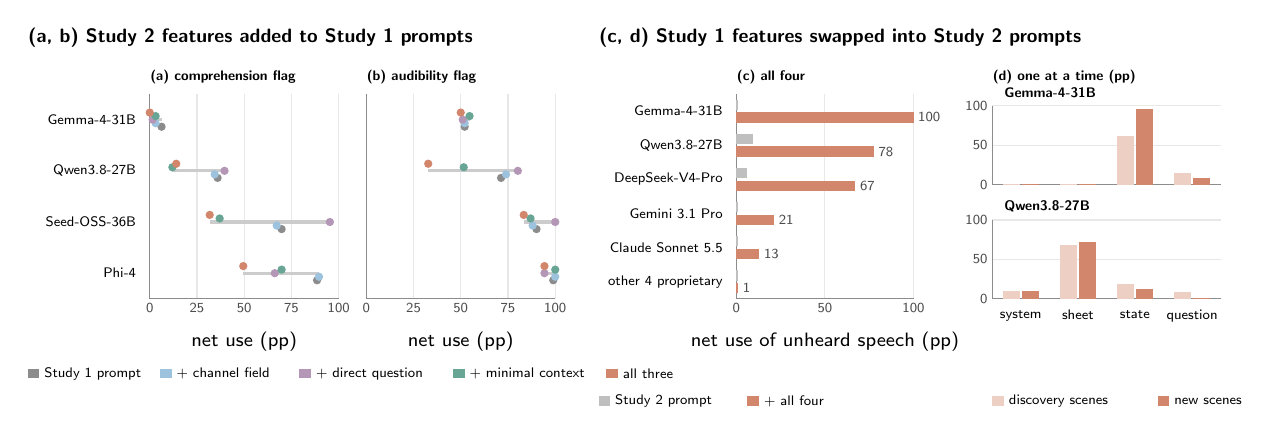
\begin{tikzpicture}[x=1cm,y=1cm]
\node[panel] at (0,3.45) {(a, b) Study 2 features added to Study 1 prompts};
\begin{scope}[xshift=1.55cm]
\node[anchor=south west,font=\sffamily\tiny\bfseries,inner sep=0pt] at (0,2.72) {(a) comprehension flag};
\draw[black!9] (0.000,0)--(0.000,2.6);
\draw[black!9] (0.600,0)--(0.600,2.6);
\draw[black!9] (1.200,0)--(1.200,2.6);
\draw[black!9] (1.800,0)--(1.800,2.6);
\draw[black!9] (2.400,0)--(2.400,2.6);
\draw[black!45,line width=.4pt] (0,2.6)--(0,0)--(2.4,0);
\node[anchor=north,font=\sffamily\tiny,text=black!70,inner sep=1.5pt] at (0.000,0) {0};
\node[anchor=north,font=\sffamily\tiny,text=black!70,inner sep=1.5pt] at (0.600,0) {25};
\node[anchor=north,font=\sffamily\tiny,text=black!70,inner sep=1.5pt] at (1.200,0) {50};
\node[anchor=north,font=\sffamily\tiny,text=black!70,inner sep=1.5pt] at (1.800,0) {75};
\node[anchor=north,font=\sffamily\tiny,text=black!70,inner sep=1.5pt] at (2.400,0) {100};
\node[anchor=north,font=\sffamily\scriptsize] at (1.2,-0.3) {net use (pp)};
\node[anchor=east,font=\sffamily\tiny] at (-0.05,2.275) {Gemma-4-31B};
\draw[black!20,line width=1.1pt] (0.000,2.275)--(0.150,2.275);
\fill[black!45] (0.150,2.185) circle (1.5pt);
\fill[OIsky] (0.075,2.230) circle (1.5pt);
\fill[OIpurple] (0.037,2.275) circle (1.5pt);
\fill[OIgreen] (0.075,2.320) circle (1.5pt);
\fill[OIorange] (0.000,2.365) circle (1.5pt);
\node[anchor=east,font=\sffamily\tiny] at (-0.05,1.625) {Qwen3.8-27B};
\draw[black!20,line width=1.1pt] (0.288,1.625)--(0.950,1.625);
\fill[black!45] (0.862,1.535) circle (1.5pt);
\fill[OIsky] (0.825,1.580) circle (1.5pt);
\fill[OIpurple] (0.950,1.625) circle (1.5pt);
\fill[OIgreen] (0.288,1.670) circle (1.5pt);
\fill[OIorange] (0.337,1.715) circle (1.5pt);
\node[anchor=east,font=\sffamily\tiny] at (-0.05,0.975) {Seed-OSS-36B};
\draw[black!20,line width=1.1pt] (0.762,0.975)--(2.288,0.975);
\fill[black!45] (1.675,0.885) circle (1.5pt);
\fill[OIsky] (1.613,0.930) circle (1.5pt);
\fill[OIpurple] (2.288,0.975) circle (1.5pt);
\fill[OIgreen] (0.888,1.020) circle (1.5pt);
\fill[OIorange] (0.762,1.065) circle (1.5pt);
\node[anchor=east,font=\sffamily\tiny] at (-0.05,0.325) {Phi-4};
\draw[black!20,line width=1.1pt] (1.188,0.325)--(2.150,0.325);
\fill[black!45] (2.125,0.235) circle (1.5pt);
\fill[OIsky] (2.150,0.280) circle (1.5pt);
\fill[OIpurple] (1.588,0.325) circle (1.5pt);
\fill[OIgreen] (1.675,0.370) circle (1.5pt);
\fill[OIorange] (1.188,0.415) circle (1.5pt);
\end{scope}
\begin{scope}[xshift=4.3cm]
\node[anchor=south west,font=\sffamily\tiny\bfseries,inner sep=0pt] at (0,2.72) {(b) audibility flag};
\draw[black!9] (0.000,0)--(0.000,2.6);
\draw[black!9] (0.600,0)--(0.600,2.6);
\draw[black!9] (1.200,0)--(1.200,2.6);
\draw[black!9] (1.800,0)--(1.800,2.6);
\draw[black!9] (2.400,0)--(2.400,2.6);
\draw[black!45,line width=.4pt] (0,2.6)--(0,0)--(2.4,0);
\node[anchor=north,font=\sffamily\tiny,text=black!70,inner sep=1.5pt] at (0.000,0) {0};
\node[anchor=north,font=\sffamily\tiny,text=black!70,inner sep=1.5pt] at (0.600,0) {25};
\node[anchor=north,font=\sffamily\tiny,text=black!70,inner sep=1.5pt] at (1.200,0) {50};
\node[anchor=north,font=\sffamily\tiny,text=black!70,inner sep=1.5pt] at (1.800,0) {75};
\node[anchor=north,font=\sffamily\tiny,text=black!70,inner sep=1.5pt] at (2.400,0) {100};
\node[anchor=north,font=\sffamily\scriptsize] at (1.2,-0.3) {net use (pp)};
\draw[black!20,line width=1.1pt] (1.200,2.275)--(1.312,2.275);
\fill[black!45] (1.250,2.185) circle (1.5pt);
\fill[OIsky] (1.250,2.230) circle (1.5pt);
\fill[OIpurple] (1.225,2.275) circle (1.5pt);
\fill[OIgreen] (1.312,2.320) circle (1.5pt);
\fill[OIorange] (1.200,2.365) circle (1.5pt);
\draw[black!20,line width=1.1pt] (0.787,1.625)--(1.925,1.625);
\fill[black!45] (1.712,1.535) circle (1.5pt);
\fill[OIsky] (1.775,1.580) circle (1.5pt);
\fill[OIpurple] (1.925,1.625) circle (1.5pt);
\fill[OIgreen] (1.238,1.670) circle (1.5pt);
\fill[OIorange] (0.787,1.715) circle (1.5pt);
\draw[black!20,line width=1.1pt] (2.000,0.975)--(2.400,0.975);
\fill[black!45] (2.162,0.885) circle (1.5pt);
\fill[OIsky] (2.113,0.930) circle (1.5pt);
\fill[OIpurple] (2.400,0.975) circle (1.5pt);
\fill[OIgreen] (2.087,1.020) circle (1.5pt);
\fill[OIorange] (2.000,1.065) circle (1.5pt);
\draw[black!20,line width=1.1pt] (2.263,0.325)--(2.400,0.325);
\fill[black!45] (2.375,0.235) circle (1.5pt);
\fill[OIsky] (2.400,0.280) circle (1.5pt);
\fill[OIpurple] (2.263,0.325) circle (1.5pt);
\fill[OIgreen] (2.400,0.370) circle (1.5pt);
\fill[OIorange] (2.263,0.415) circle (1.5pt);
\end{scope}
\fill[black!45] (0.000,-1.010) rectangle (0.150,-0.890);
\node[anchor=west,font=\sffamily\tiny,inner sep=1pt] at (0.170,-0.950) {Study 1 prompt};
\fill[OIsky] (1.680,-1.010) rectangle (1.830,-0.890);
\node[anchor=west,font=\sffamily\tiny,inner sep=1pt] at (1.850,-0.950) {+ channel field};
\fill[OIpurple] (3.450,-1.010) rectangle (3.600,-0.890);
\node[anchor=west,font=\sffamily\tiny,inner sep=1pt] at (3.620,-0.950) {+ direct question};
\fill[OIgreen] (5.400,-1.010) rectangle (5.550,-0.890);
\node[anchor=west,font=\sffamily\tiny,inner sep=1pt] at (5.570,-0.950) {+ minimal context};
\fill[OIorange] (7.350,-1.010) rectangle (7.500,-0.890);
\node[anchor=west,font=\sffamily\tiny,inner sep=1pt] at (7.520,-0.950) {all three};
\begin{scope}[xshift=9.0cm]
\node[panel] at (-1.75,3.45) {(c, d) Study 1 features swapped into Study 2 prompts};
\node[anchor=south west,font=\sffamily\tiny\bfseries,inner sep=0pt] at (0,2.72) {(c) all four};
\draw[black!9] (0.000,0)--(0.000,2.6);
\draw[black!9] (1.125,0)--(1.125,2.6);
\draw[black!9] (2.250,0)--(2.250,2.6);
\draw[black!45,line width=.4pt] (0,2.6)--(0,0)--(2.25,0);
\node[anchor=north,font=\sffamily\tiny,text=black!70,inner sep=1.5pt] at (0.000,0) {0};
\node[anchor=north,font=\sffamily\tiny,text=black!70,inner sep=1.5pt] at (1.125,0) {50};
\node[anchor=north,font=\sffamily\tiny,text=black!70,inner sep=1.5pt] at (2.250,0) {100};
\node[anchor=north,font=\sffamily\scriptsize] at (1.125,-0.3) {net use of unheard speech (pp)};
\node[anchor=east,font=\sffamily\tiny] at (-0.05,2.383) {Gemma-4-31B};
\fill[black!25] (0,2.398) rectangle (0.020,2.528);
\fill[OIorange] (0,2.238) rectangle (2.250,2.368);
\node[anchor=west,font=\sffamily\tiny,text=black!70,inner sep=1.5pt] at (2.250,2.303) {100};
\node[anchor=east,font=\sffamily\tiny] at (-0.05,1.950) {Qwen3.8-27B};
\fill[black!25] (0,1.965) rectangle (0.211,2.095);
\fill[OIorange] (0,1.805) rectangle (1.746,1.935);
\node[anchor=west,font=\sffamily\tiny,text=black!70,inner sep=1.5pt] at (1.746,1.870) {78};
\node[anchor=east,font=\sffamily\tiny] at (-0.05,1.517) {DeepSeek-V4-Pro};
\fill[black!25] (0,1.532) rectangle (0.141,1.662);
\fill[OIorange] (0,1.372) rectangle (1.512,1.502);
\node[anchor=west,font=\sffamily\tiny,text=black!70,inner sep=1.5pt] at (1.512,1.437) {67};
\node[anchor=east,font=\sffamily\tiny] at (-0.05,1.083) {Gemini 3.1 Pro};
\fill[black!25] (0,1.098) rectangle (0.020,1.228);
\fill[OIorange] (0,0.938) rectangle (0.480,1.068);
\node[anchor=west,font=\sffamily\tiny,text=black!70,inner sep=1.5pt] at (0.480,1.003) {21};
\node[anchor=east,font=\sffamily\tiny] at (-0.05,0.650) {Claude Sonnet 5.5};
\fill[black!25] (0,0.665) rectangle (0.020,0.795);
\fill[OIorange] (0,0.505) rectangle (0.293,0.635);
\node[anchor=west,font=\sffamily\tiny,text=black!70,inner sep=1.5pt] at (0.293,0.570) {13};
\node[anchor=east,font=\sffamily\tiny] at (-0.05,0.217) {other 4 proprietary};
\fill[black!25] (0,0.232) rectangle (0.020,0.362);
\fill[OIorange] (0,0.072) rectangle (0.023,0.202);
\node[anchor=west,font=\sffamily\tiny,text=black!70,inner sep=1.5pt] at (0.023,0.137) {1};
\fill[black!25] (-1.750,-1.360) rectangle (-1.600,-1.240);
\node[anchor=west,font=\sffamily\tiny,inner sep=1pt] at (-1.580,-1.300) {Study 2 prompt};
\fill[OIorange] (0.140,-1.360) rectangle (0.290,-1.240);
\node[anchor=west,font=\sffamily\tiny,inner sep=1pt] at (0.310,-1.300) {+ all four};
\end{scope}
\begin{scope}[xshift=12.25cm]
\node[anchor=south west,font=\sffamily\tiny\bfseries,inner sep=0pt] at (0,2.72) {(d) one at a time (pp)};
\begin{scope}[yshift=1.450cm]
\draw[black!9] (0,0.000)--(2.9,0.000);
\draw[black!9] (0,0.500)--(2.9,0.500);
\draw[black!9] (0,1.000)--(2.9,1.000);
\draw[black!45,line width=.4pt] (0,1.0000000000000002)--(0,0)--(2.9,0);
\node[anchor=east,font=\sffamily\tiny,text=black!70,inner sep=1.5pt] at (0,0.000) {0};
\node[anchor=east,font=\sffamily\tiny,text=black!70,inner sep=1.5pt] at (0,0.500) {50};
\node[anchor=east,font=\sffamily\tiny,text=black!70,inner sep=1.5pt] at (0,1.000) {100};
\node[anchor=south west,font=\sffamily\tiny\bfseries] at (0.03,0.980) {Gemma-4-31B};
\fill[OIorange!40] (0.133,0) rectangle (0.352,0.008);
\fill[OIorange] (0.372,0) rectangle (0.593,0.008);
\fill[OIorange!40] (0.857,0) rectangle (1.077,0.010);
\fill[OIorange] (1.097,0) rectangle (1.318,0.008);
\fill[OIorange!40] (1.582,0) rectangle (1.802,0.615);
\fill[OIorange] (1.823,0) rectangle (2.042,0.958);
\fill[OIorange!40] (2.308,0) rectangle (2.527,0.141);
\fill[OIorange] (2.548,0) rectangle (2.768,0.083);
\end{scope}
\begin{scope}[yshift=0.000cm]
\draw[black!9] (0,0.000)--(2.9,0.000);
\draw[black!9] (0,0.500)--(2.9,0.500);
\draw[black!9] (0,1.000)--(2.9,1.000);
\draw[black!45,line width=.4pt] (0,1.0000000000000002)--(0,0)--(2.9,0);
\node[anchor=east,font=\sffamily\tiny,text=black!70,inner sep=1.5pt] at (0,0.000) {0};
\node[anchor=east,font=\sffamily\tiny,text=black!70,inner sep=1.5pt] at (0,0.500) {50};
\node[anchor=east,font=\sffamily\tiny,text=black!70,inner sep=1.5pt] at (0,1.000) {100};
\node[anchor=south west,font=\sffamily\tiny\bfseries] at (0.03,0.980) {Qwen3.8-27B};
\fill[OIorange!40] (0.133,0) rectangle (0.352,0.099);
\fill[OIorange] (0.372,0) rectangle (0.593,0.104);
\node[anchor=north,font=\sffamily\tiny] at (0.362,-0.02) {system};
\fill[OIorange!40] (0.857,0) rectangle (1.077,0.677);
\fill[OIorange] (1.097,0) rectangle (1.318,0.719);
\node[anchor=north,font=\sffamily\tiny] at (1.087,-0.02) {sheet};
\fill[OIorange!40] (1.582,0) rectangle (1.802,0.193);
\fill[OIorange] (1.823,0) rectangle (2.042,0.125);
\node[anchor=north,font=\sffamily\tiny] at (1.812,-0.02) {state};
\fill[OIorange!40] (2.308,0) rectangle (2.527,0.089);
\fill[OIorange] (2.548,0) rectangle (2.768,0.008);
\node[anchor=north,font=\sffamily\tiny] at (2.538,-0.02) {question};
\end{scope}
\fill[OIorange!40] (0.000,-1.360) rectangle (0.150,-1.240);
\node[anchor=west,font=\sffamily\tiny,inner sep=1pt] at (0.170,-1.300) {discovery scenes};
\fill[OIorange] (2.100,-1.360) rectangle (2.250,-1.240);
\node[anchor=west,font=\sffamily\tiny,inner sep=1pt] at (2.270,-1.300) {new scenes};
\end{scope}
\end{tikzpicture}
\end{document}
